\chapter{Circuiti RC e RL (C3)}

Oggetto di studio di questa esperienza è l'andamento della differenza di potenziale ai capi di resistenza e capacità o induttanza.
A tal fine costruiamo un circuito con i seguenti elementi:
[disegno]

\begin{itemize}
  \item Generatore di onde
  \item Un condensatore di capacità 367 $nF$
  \item Un'induttore di induttanza sconosciuta, e resistenza 40 $\Omega$.
  \item Un oscilloscopio con due sonde
  \item Una resistenza di 667 $\Omega$ (più errore)
\end{itemize}

\section{Corrente impulsata}
\subsection{Procedimento}


Per simulare l'apertura e la chiusura del circuito impostiamo nel generatore la modalità onda quadra. Una sonda posta prima del condensatore mostra sullo schermo dell'oscilloscopio il segnale.  
Una seconda sonda, posta ai capi della resistenza, visualizza la forma dell'onda caratteristica della carica o della scarica di un condensatore/induttore.




\subsection{Dati} 

\subsubsection{Circuito RC}

Raccogliamo i dati (differenza di potenziale e tempo) dall'onda visualizzata sul display dell'oscilloscopio, tramite i cursori. 

Con un'onda quadra a 50 Hz, abbiamo raccolto i seguenti dati:
\begin{center}
\begin{tabular}{*{2}{c}}
Tempo ($\mu s$) & Ddp ($V$) \\
\midrule
0 & 18.20 \\
100 & 12.80 \\
200 & 9.00 \\
300 & 5.80 \\
400 & 4.40 \\
500 & 3.20 \\
600 & 2.20 \\
700 & 1.80 \\
800 & 1.20 \\
900 & 1.00 \\
\end{tabular}
\end{center}

Interpoliamo i dati raccolti con la curva caratteristica della carica di un condensatore: 
$$V_R = \varepsilon e^{-t/\tau}$$

Il valore stimato dall'interpolazione è $\tau=281.7 \pm 5 \mu s$.
Valore atteso: $\tau=RC=248.5 \mu s$


\begin{center}
 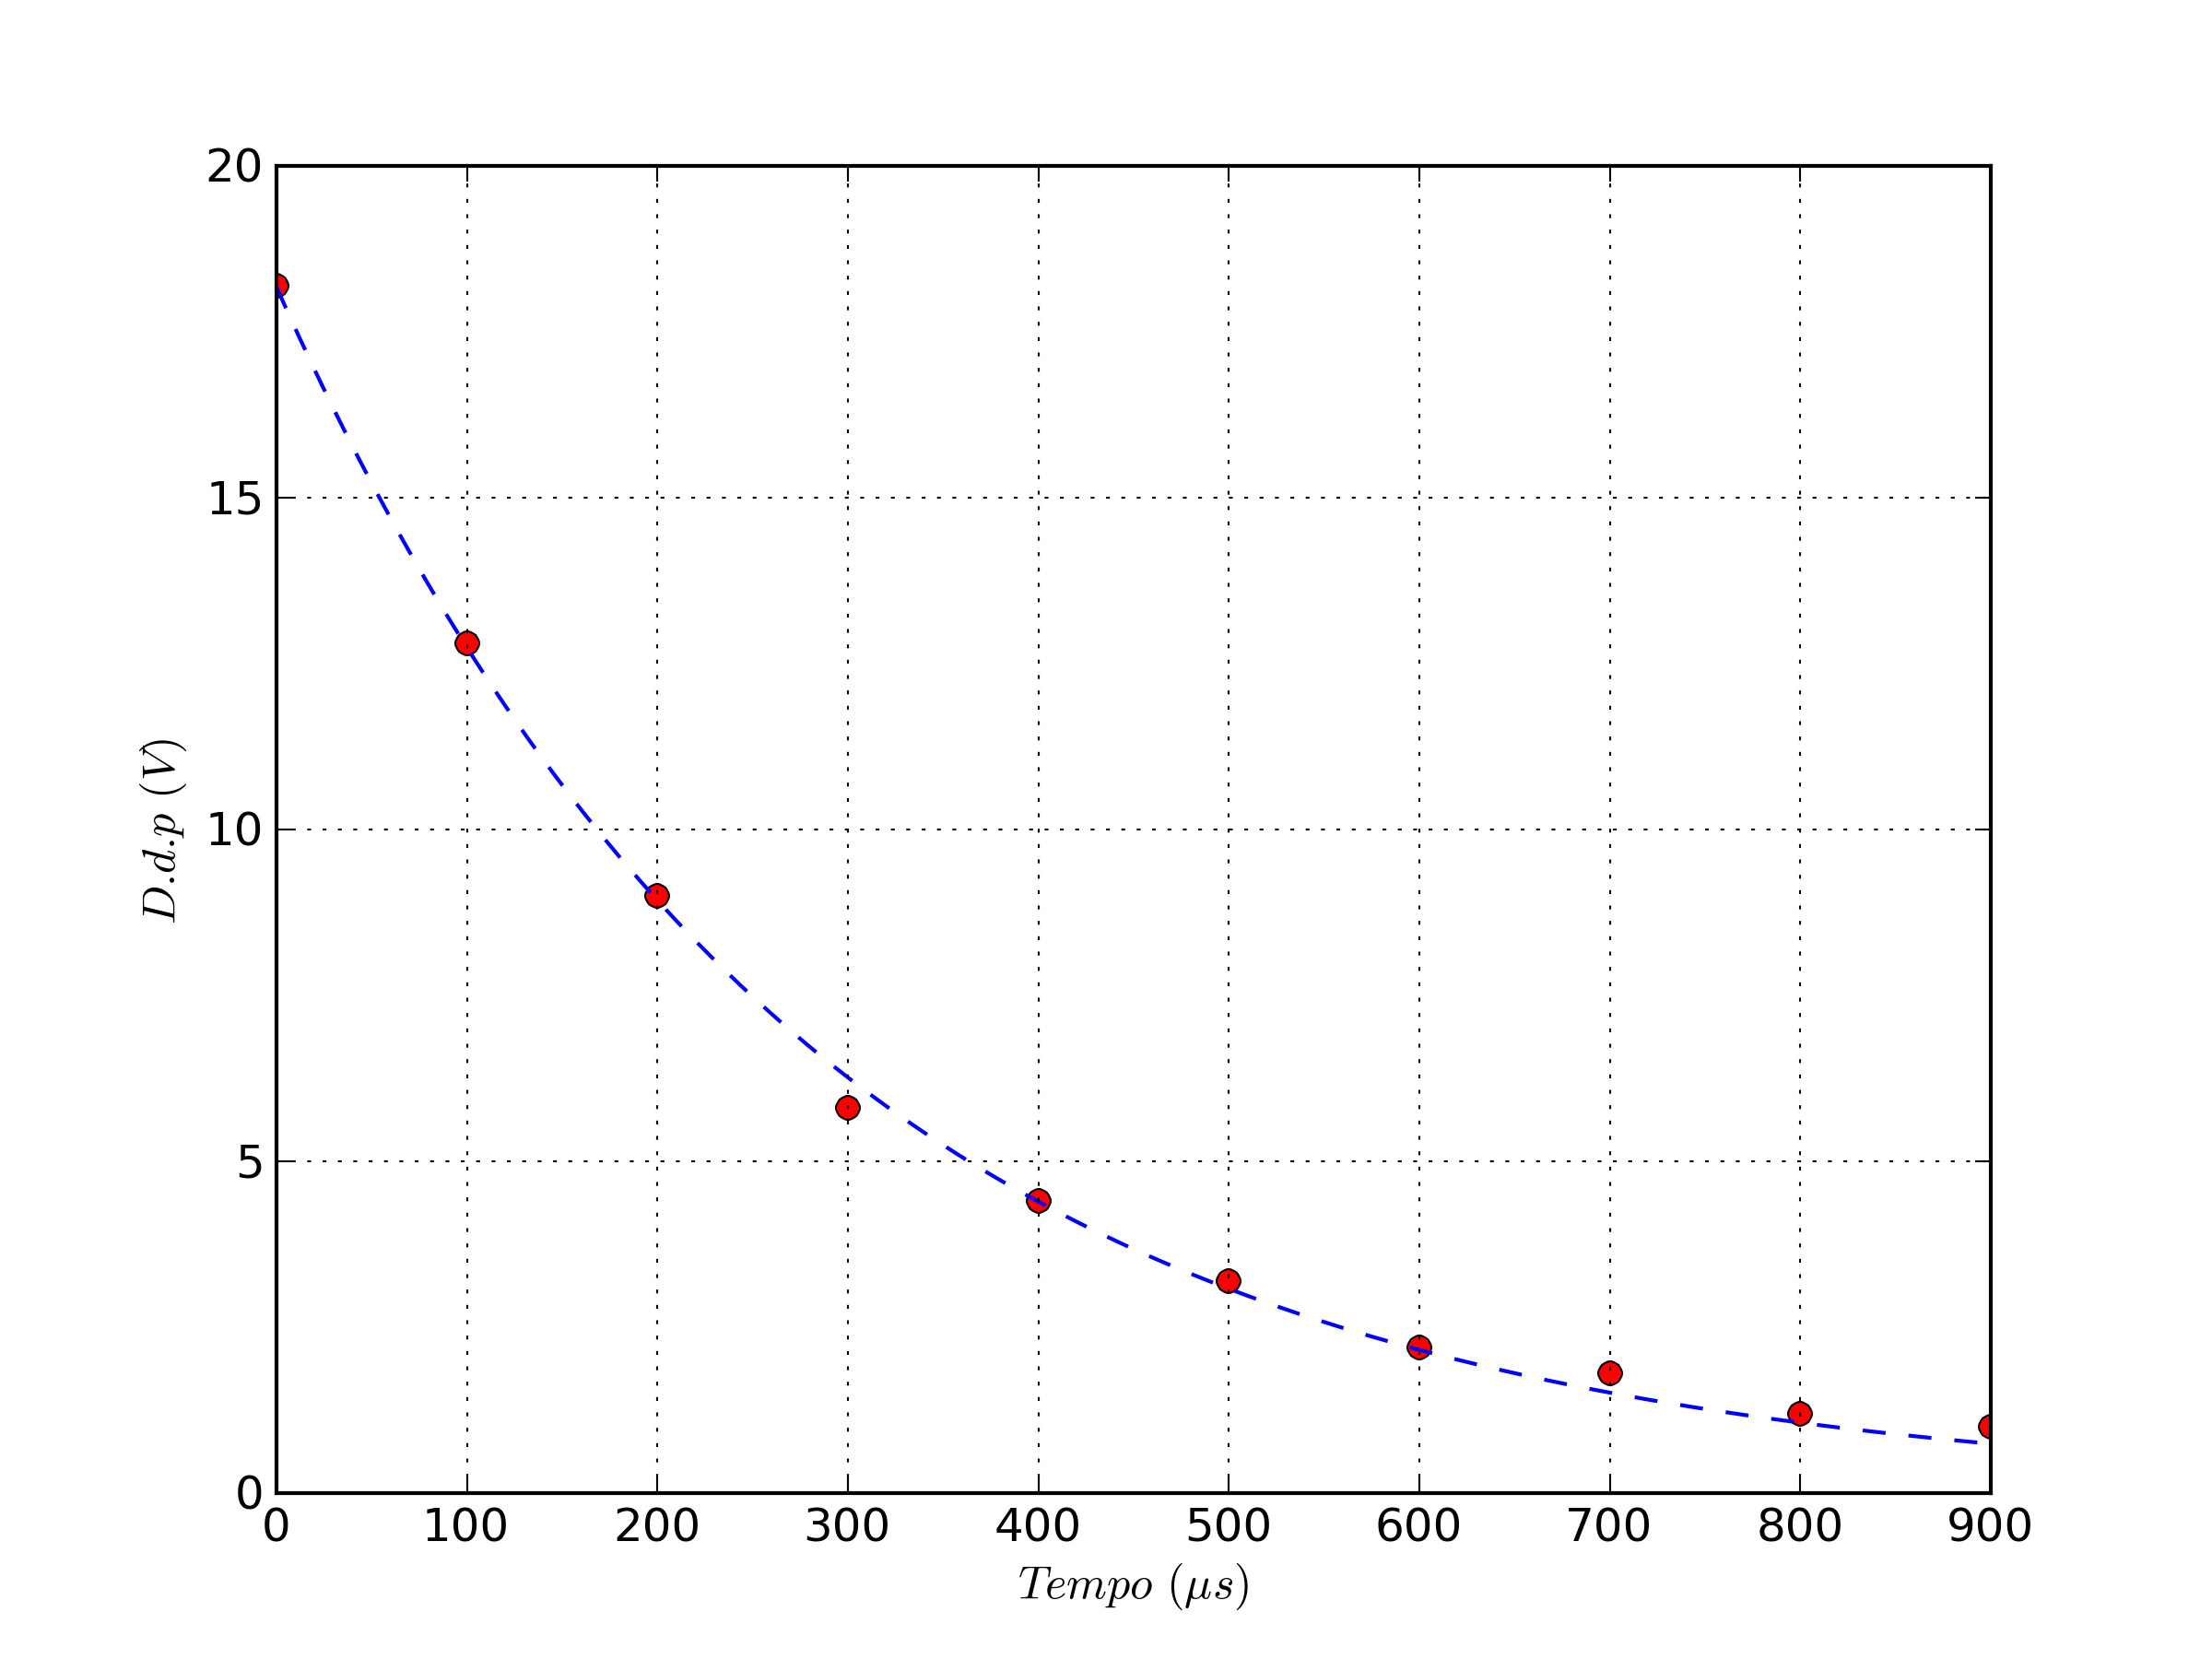
\includegraphics[scale=0.70]{grafici/C3/fitcond.png}
\end{center}

%chi quadro!



\subsubsection{Circuito RL}
Con un'onda quadra a 250 Hz, abbiamo raccolto i seguenti dati:

\begin{center}
\begin{tabular}{*{2}{c}}
Tempo ($\mu s$) & Ddp ($V$) \\
\midrule
5 & 5.00 \\
10 & 8.00 \\
15 & 10.60 \\
20 & 12.40 \\
25 & 13.60 \\
30 & 14.60 \\
35 & 15.40 \\
40 & 16.20 \\
45 & 16.40 \\
\end{tabular}
\end{center}
Interpoliamo i dati raccolti con la curva caratteristica della carica del circuito:

$$V_R = \varepsilon \left( 1-e^{-t/\tau} \right)$$

Il valore stimato dall'interpolazione è $\tau=16.05 \mu s$ \\
Non conoscendo a priori il valore di L non possiamo valutare l'accordo con il valore teorico: $\tau=\frac{L}{R}$.

\begin{center}
 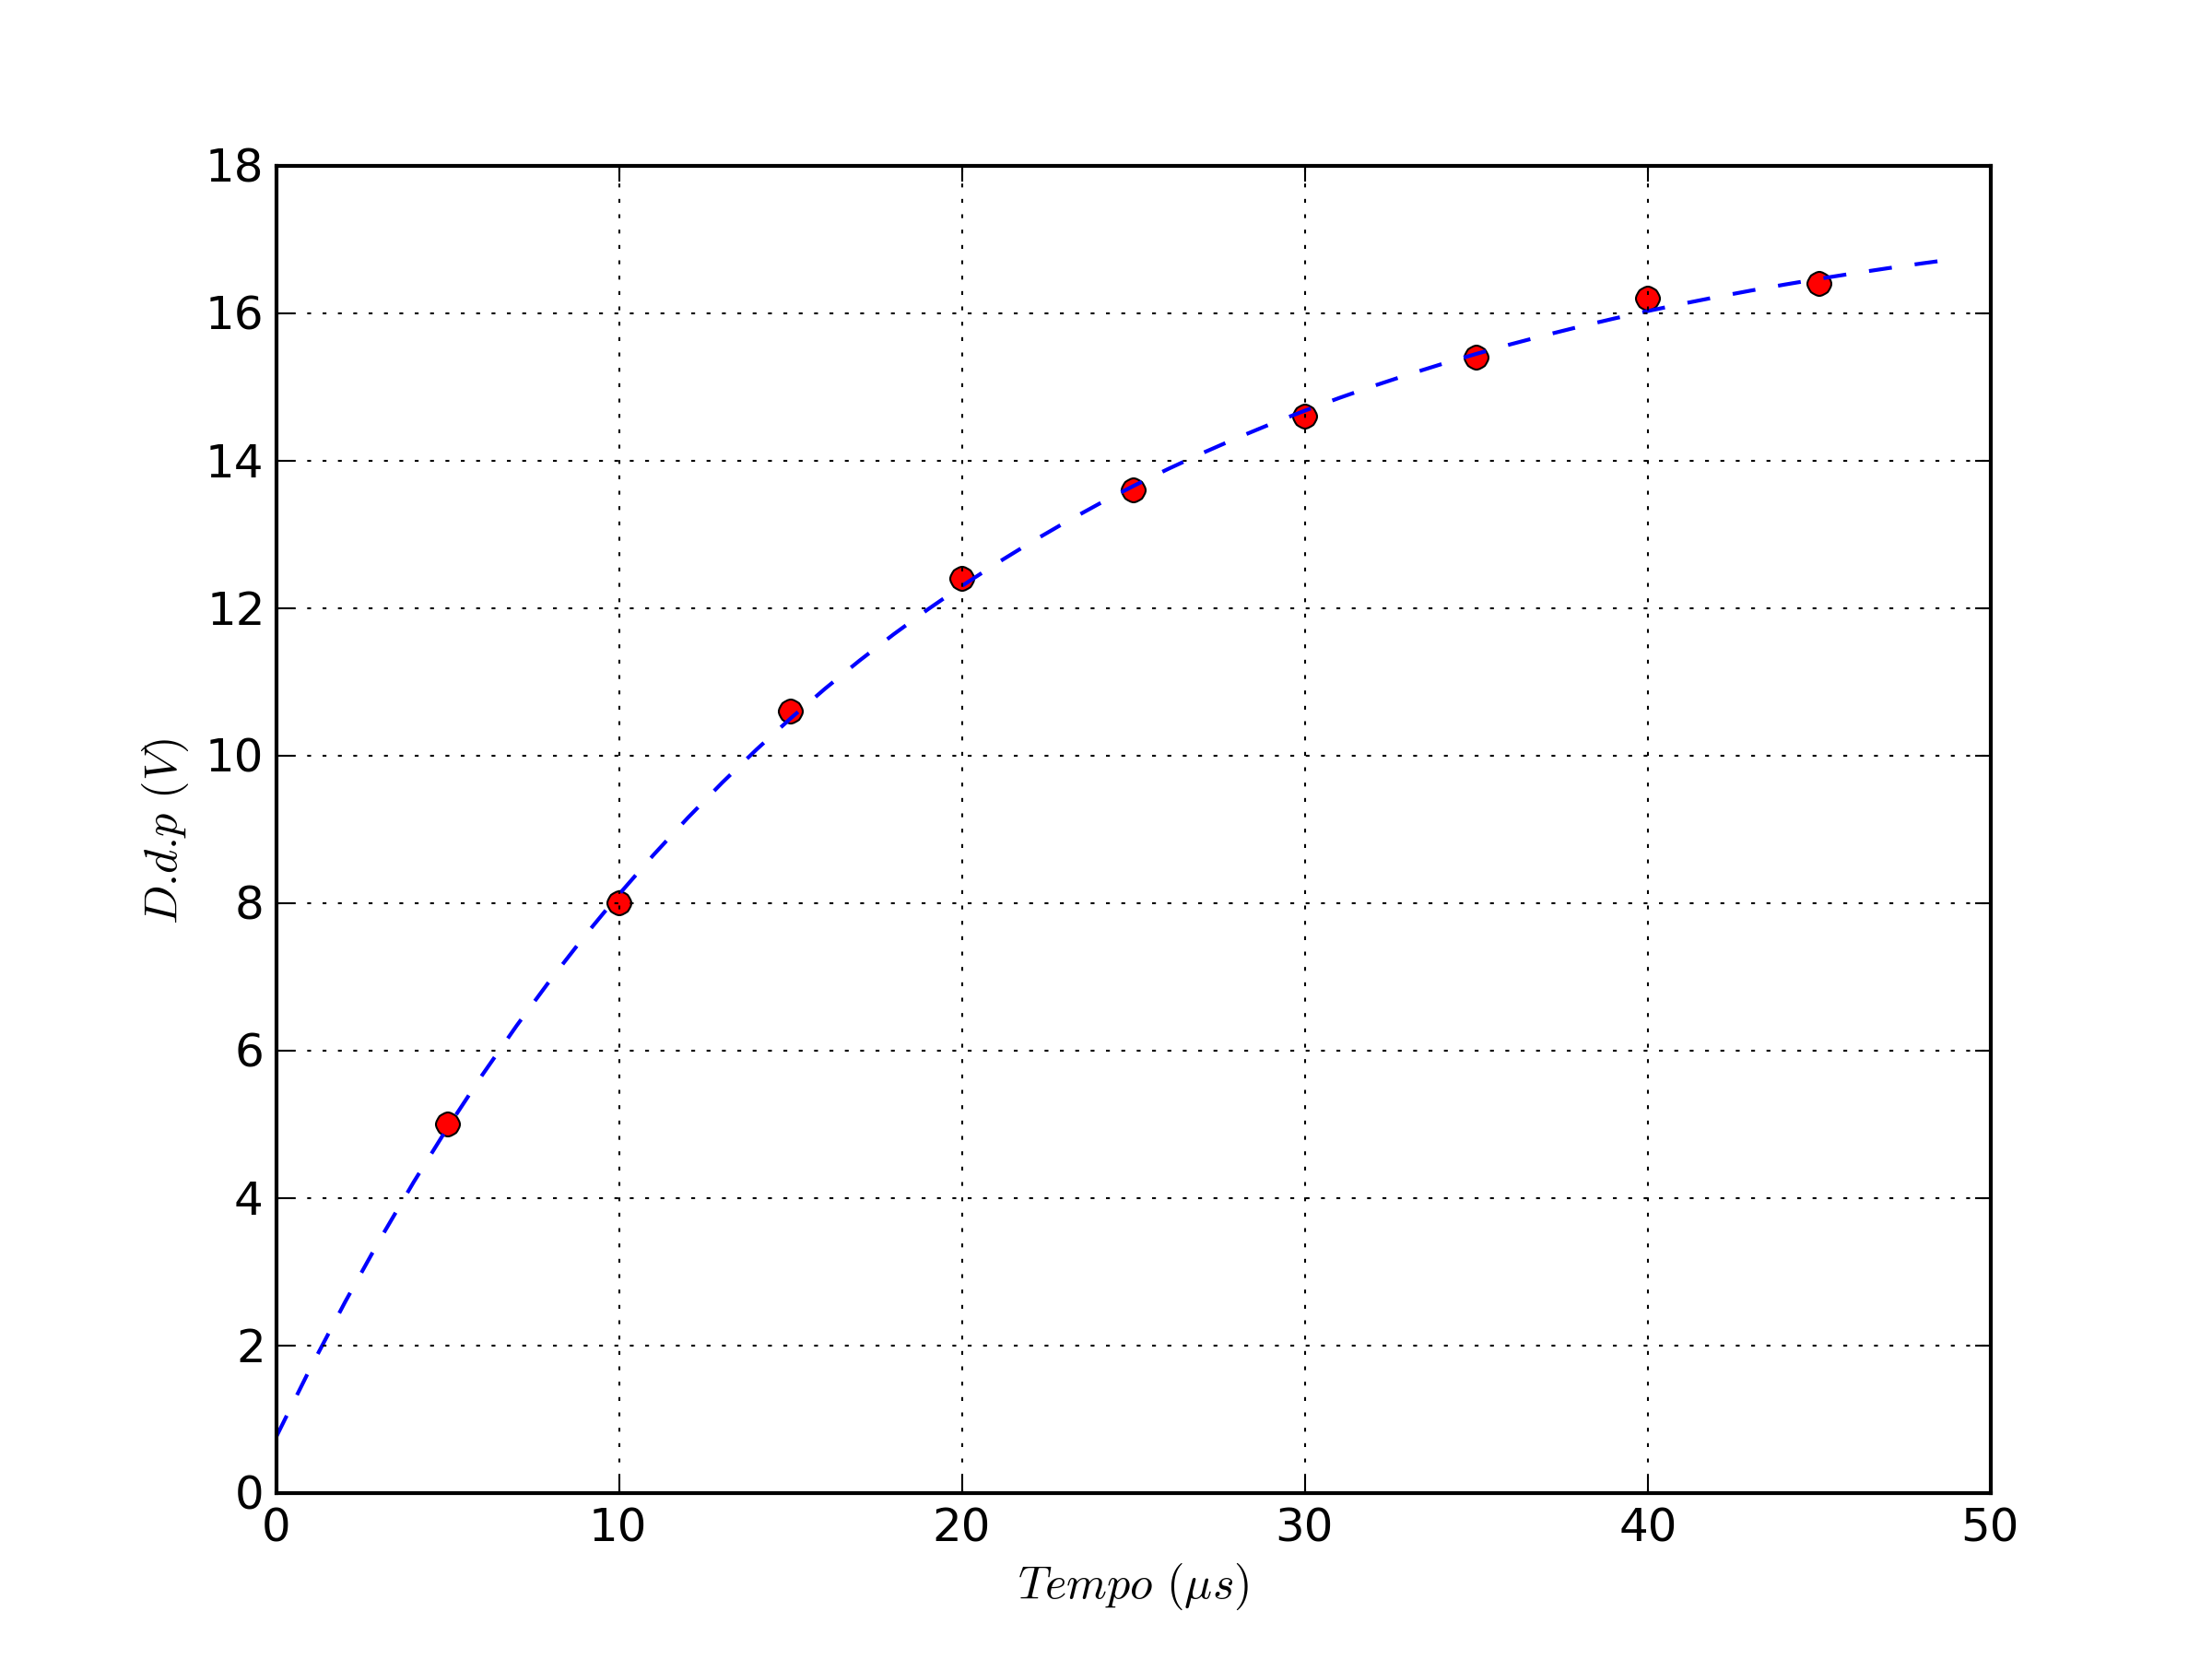
\includegraphics[scale=0.70]{grafici/C3/fitindu.png}
\end{center}

%chi quadro!



\section{Corrente alternata}
\subsection{Procedimento}
Nella seconda parte dell'esperienza intendiamo misurare la risposta in frequenza (o funzione di trasferimento), definita come:

$H\left(\omega \right) = $  


Pertanto misuriamo la ddp ai capi di $R$ e $C$ o $L$ in modo analogo alle prima parte dell'esperienza, e la distanza tra due picchi delle onde visualizzate a schermo per determinare l'angolo $\phi$ di sfasamento.

Per ricavare il rapporto $\frac{V_{R}}{V_{o}}$, dobbiamo ricavare $V_R$. Trovandoci in regime di corrente alternata, la leggge di Ohm è nella forma: $ V_o = Zi_o$ con $Z = R + jX$, impedenza del circuito.
Trattandosi di circuiti RC e RL in cui le impedenze sono collegate in serie, si ha $Z_{tot} = \sum Z_i$

\begin{itemize}
\item circuito RC $\rightarrow$ $Z=R-\frac{j}{\omega C}$
\item circuito RL $\rightarrow$ $Z=R+j\omega L$
\end{itemize}  

Allora: 


$$V_{Ro} = Ri_o = \frac{V_o}{Z} = \frac{RV_o}{\sqrt{R^2+X^2}} $$

$$\frac{V_{Ro}}{V_o} = \frac{R}{\sqrt{R^2+(\omega L)^2}}$$

$$\frac{V_{Ro}}{V_o} = \frac{R}{\sqrt{R^2+(\omega C)^{-2}}}$$

$$\phi = \arctan \frac{X}{R} $$

\subsection{Raccolta dati}

\subsubsection{Circuito RC}

\begin{center}
 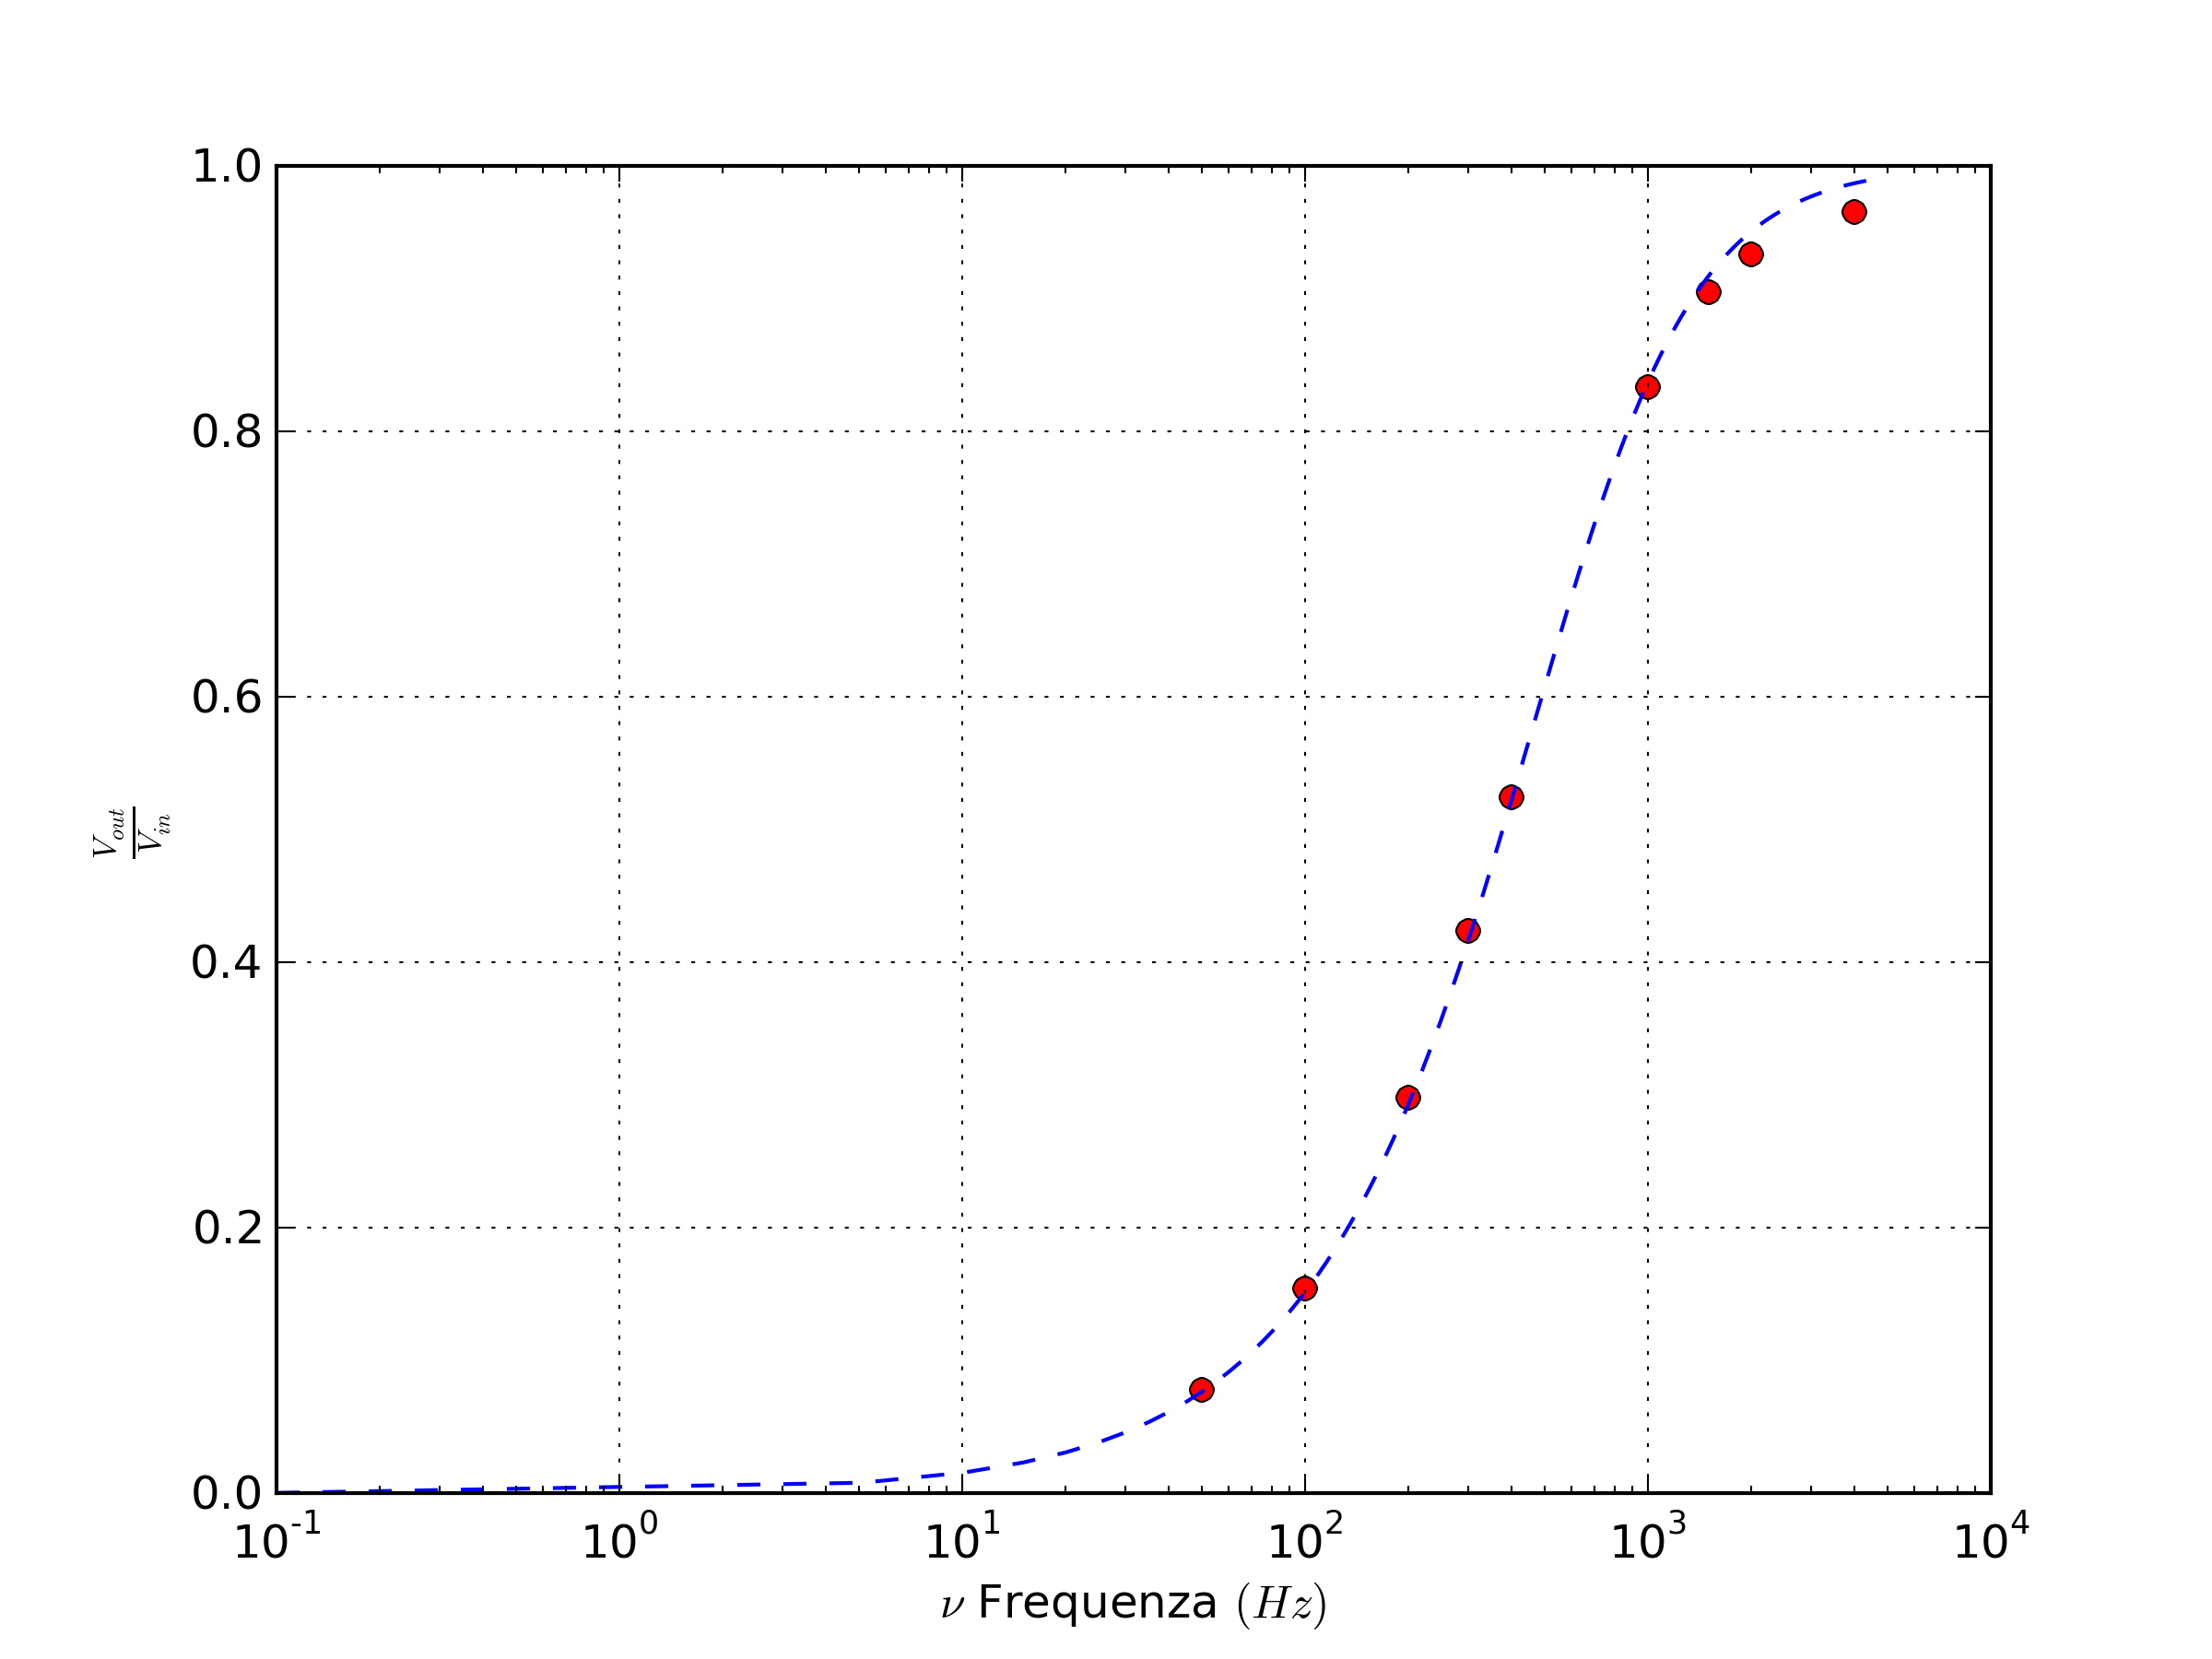
\includegraphics[scale=0.70]{grafici/C3/ddpcond.png}
\end{center}

\begin{center}
\begin{tabular}{*{2}{c}}
Frequenza ($Hz$) & Delta V ($V_{out}/V_{in}$) \\
\midrule
50 & 0.08 \\
100 & 0.15 \\
200 & 0.30 \\
300 & 0.42 \\
400 & 0.52 \\
1000 & 0.83 \\
1500 & 0.90 \\
2000 & 0.93 \\
4000 & 0.97 \\
\end{tabular}
\end{center}


\subsubsection{Circuito RL}

\begin{center}
 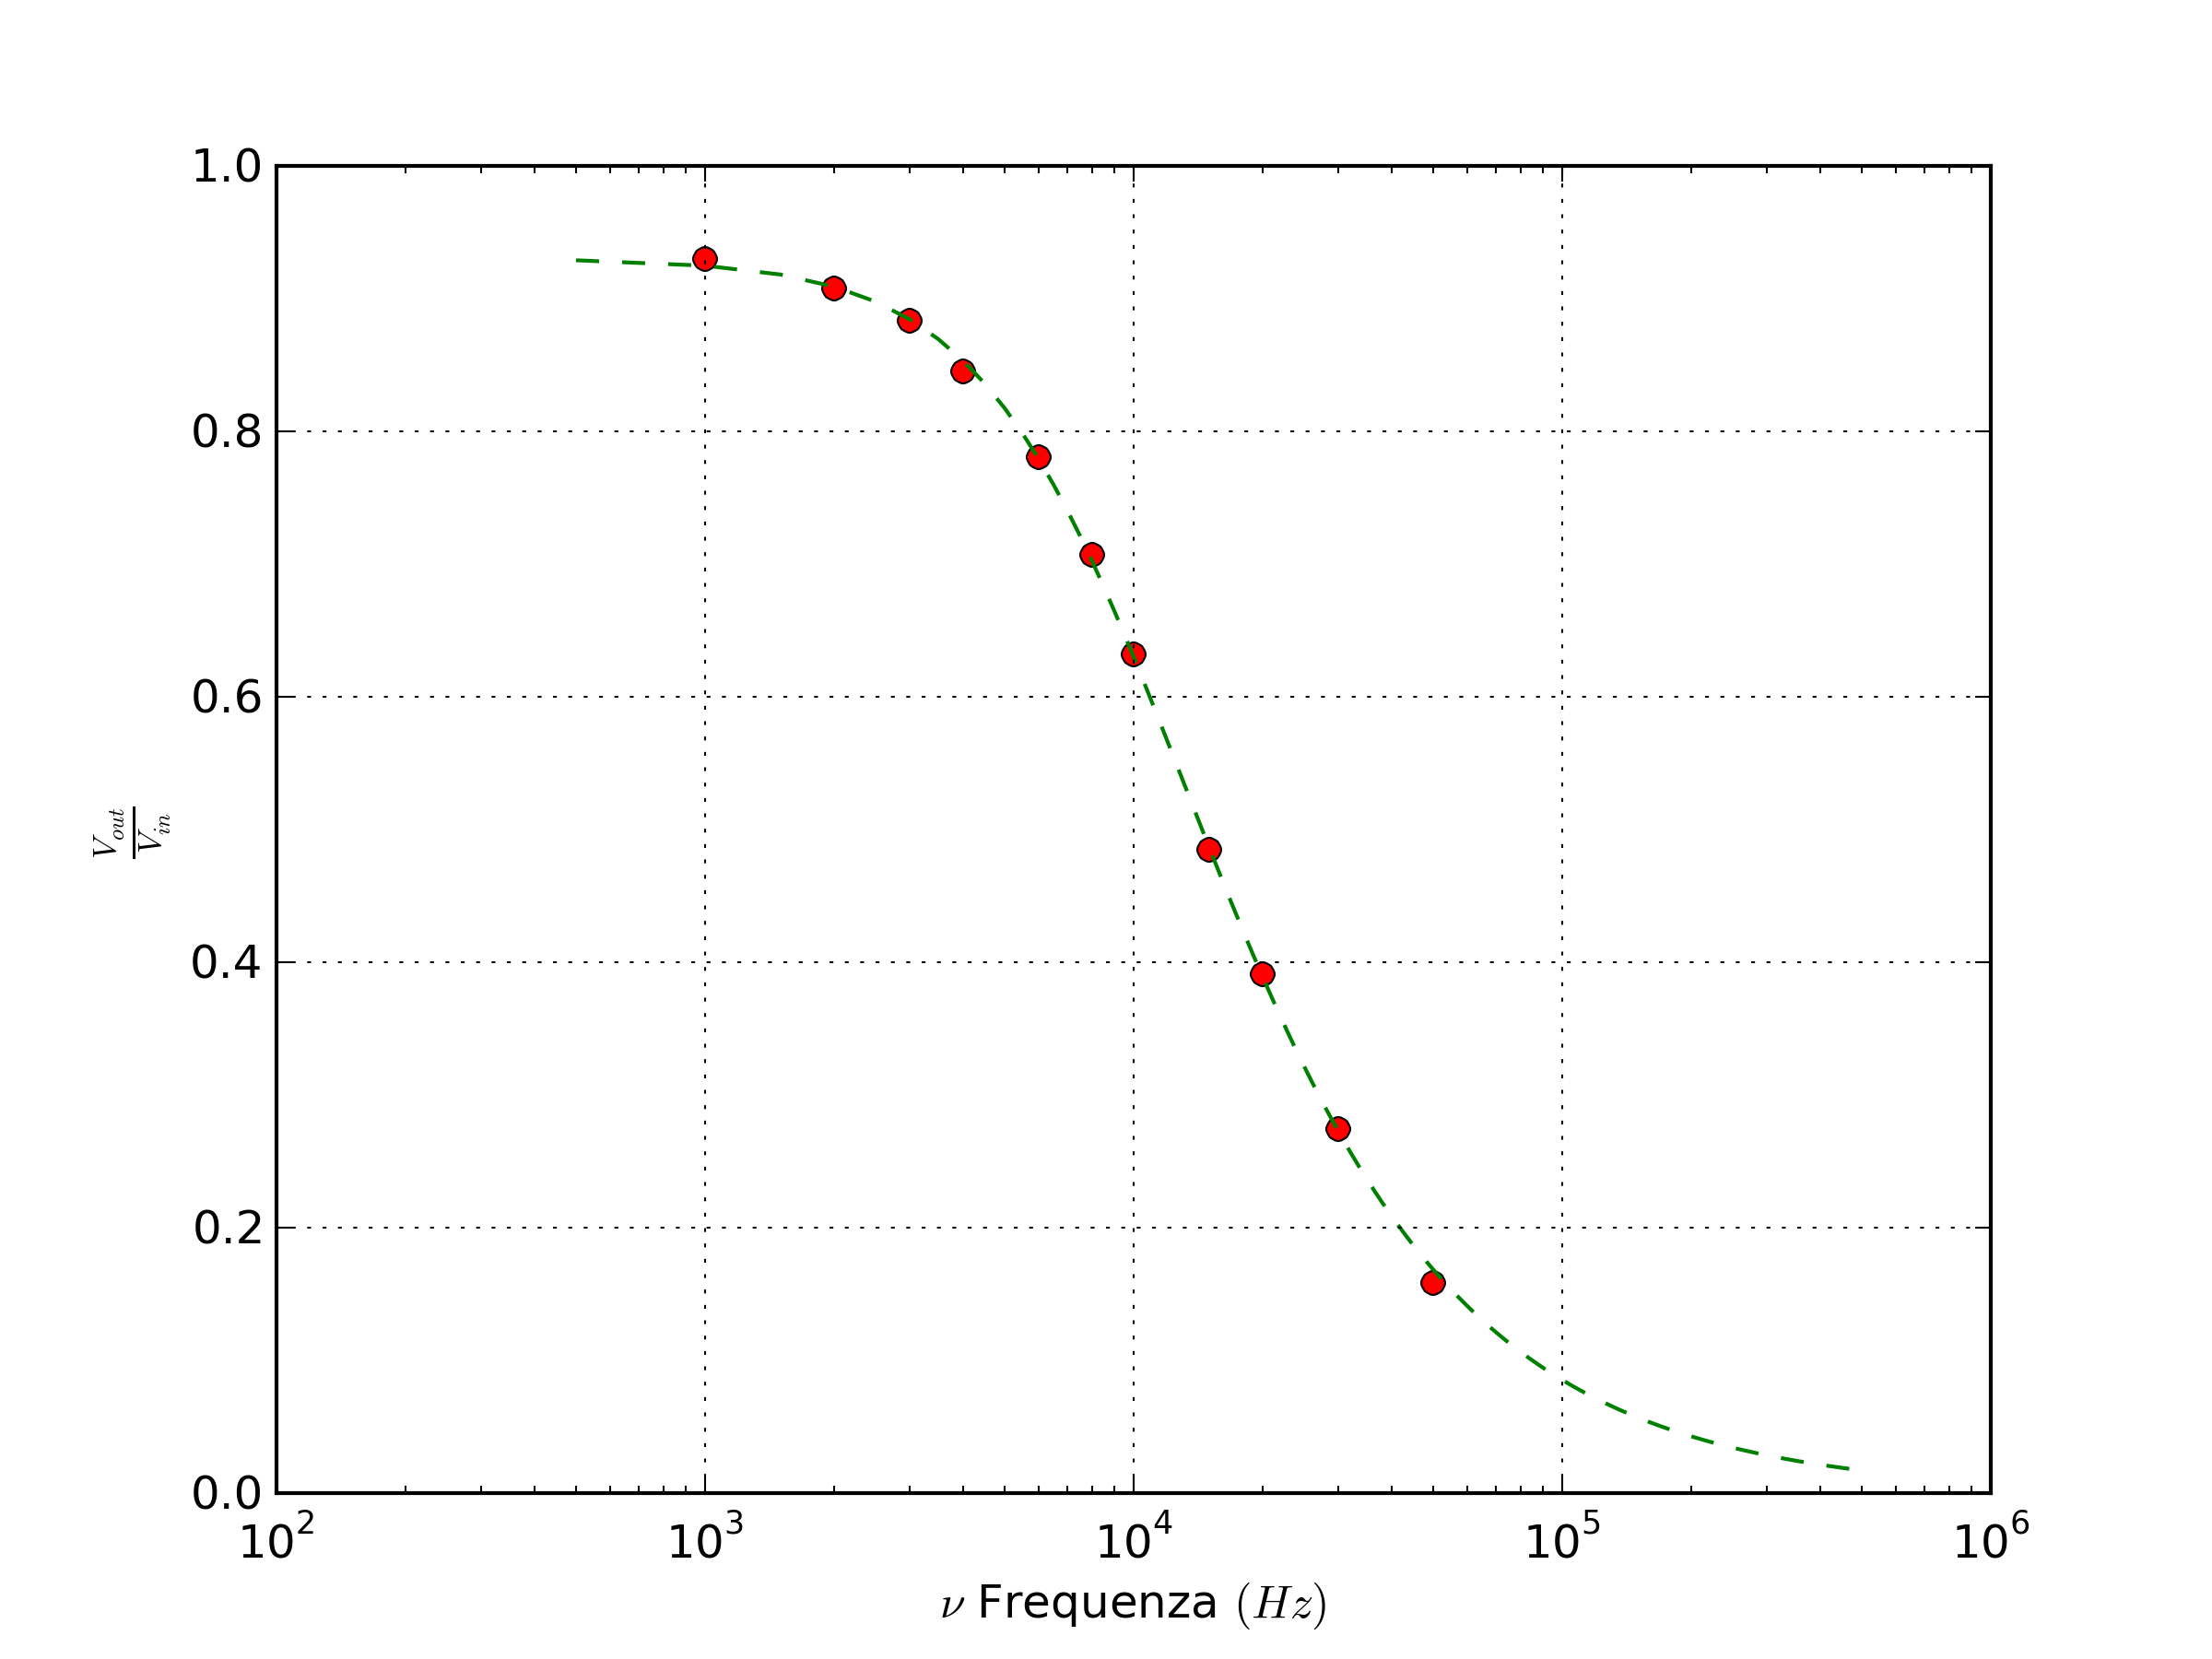
\includegraphics[scale=0.70]{grafici/C3/ddpindu.png}
\end{center}

\begin{center}
\begin{tabular}{*{2}{c}}
Frequenza ($Hz$) & Delta V ($V_{out}/V_{in}$) \\
\midrule
50 & 0.08 \\
100 & 0.15 \\
200 & 0.30 \\
300 & 0.42 \\
400 & 0.52 \\
1000 & 0.83 \\
1500 & 0.90 \\
2000 & 0.93 \\
4000 & 0.97 \\
\end{tabular}
\end{center}

\section{Conclusioni}
\subsubsection{Circuito RC}
\subsubsection{Circuito RL}
